%% Artículo del Entregable 3 en la plantilla Springer Nature (sn-jnl), con la estructura del ejemplo de la
%% guía: título, resumen, palabras clave, introducción, metodología (datos y ETL/EDA, modelos de referencia,
%% modelo propuesto, configuración experimental), resultados, conclusiones, declaraciones y referencias.
%% Las tablas (tablas/) y las figuras (figuras/) las genera generar_material.py a partir de los resultados
%% del proyecto; se compila con compilar.py.
\documentclass[pdflatex,sn-mathphys-num]{sn-jnl}

\usepackage{graphicx}
\usepackage{multirow}
\usepackage{amsmath,amssymb,amsfonts}
\usepackage{amsthm}
\usepackage{mathrsfs}
\usepackage[title]{appendix}
\usepackage{xcolor}
\usepackage{textcomp}
\usepackage{manyfoot}
\usepackage{booktabs}
\usepackage{algorithm}
\usepackage{algorithmicx}
\usepackage{algpseudocode}
\usepackage{listings}
\usepackage{array}
\usepackage[T1]{fontenc}
\usepackage[spanish,es-tabla,es-noshorthands,es-nolayout]{babel}

\graphicspath{{figuras/}}
\newcommand{\ap}{\texttt{active\_products}}
\newcommand{\cp}{\texttt{churn\_probability}}

\begin{document}

\title[EBM para la fuga de clientes en una fintech colombiana]{Clasificación y regresión de la fuga de clientes en una fintech colombiana (COFINFAD) con una \textit{Explainable Boosting Machine}: un modelo aditivo interpretable que supera a los modelos lineales previos e iguala al \textit{gradient boosting}}

\author[1]{\fnm{Valerie} \sur{Martínez Pulido}}\email{pmartinezv@uninorte.edu.co}
\author[1]{\fnm{Abrahan} \sur{Basto Martínez}}\email{abrahanb@uninorte.edu.co}
\author*[1]{\fnm{Rubén} \sur{Esguerra Fernández}}\email{esguerrar@uninorte.edu.co}

\affil*[1]{\orgdiv{Departamento de Matemáticas, Física y Ciencia de Datos}, \orgname{Universidad del Norte}, \orgaddress{\city{Barranquilla}, \country{Colombia}}}

\abstract{La fuga de clientes es uno de los problemas de predicción más frecuentes en los servicios financieros digitales, y su modelado depende tanto de la calidad de los datos como de la capacidad del modelo para captar relaciones no lineales. Sobre el conjunto público COFINFAD (48.723 clientes de una \textit{fintech} colombiana, 54 variables y 3,16 millones de transacciones de 2023) se abordan la clasificación del cuarto de clientes de mayor riesgo y la regresión de la probabilidad de fuga. Se propone una \textit{Explainable Boosting Machine} (EBM), un modelo aditivo generalizado cuyas funciones de forma se aprenden por \textit{boosting} cíclico de árboles pequeños, adaptada con pesos de clase y con una búsqueda de hiperparámetros multi-fidelidad, y se compara con los ocho modelos del curso (k-NN, Naive Bayes, regresión logística, Ridge y Lasso, árbol de decisión, Random Forest, XGBoost y SVM) dentro de un pipeline de 140 corridas con validación cruzada anidada y cuatro métodos de optimización de hiperparámetros. En la partición y etiqueta de la entrega anterior, la EBM eleva el AUC de 0,6832 a 0,7187 (DeLong, $p<10^{-18}$) y el $R^2$ de 0,1511 a 0,2159 (Diebold-Mariano, $p<10^{-39}$); frente a todos los modelos de referencia obtiene el mayor AUC de prueba (0,8289), sin diferencias significativas con los modelos de árboles, y queda a dos milésimas del techo de información de los datos. Su inferencia sobre los 9.745 clientes de prueba tarda 0,07 s, como XGBoost, pero su ajuste (27 s) es unas 16 veces más lento, lo que se reporta y discute. La EBM ofrece la precisión del \textit{boosting} con la legibilidad de un modelo aditivo.}

\keywords{Explainable Boosting Machine, fuga de clientes, clasificación y regresión, fintech, AUC, validación cruzada anidada}

\maketitle

\section{Introducción}\label{sec:intro}

Retener a un cliente cuesta menos que conseguir uno nuevo, y por eso la predicción de la fuga (\textit{churn}) es una de las aplicaciones más extendidas del aprendizaje supervisado en banca, telecomunicaciones y servicios digitales \cite{verbeke2012churn}. En una \textit{fintech} casi toda la relación con el cliente deja huella digital (uso de la aplicación, tenencia de productos, satisfacción declarada y actividad transaccional), y un modelo capaz de ordenar a los clientes por su riesgo de abandono permite concentrar una campaña de retención, de presupuesto limitado, en quienes más la necesitan.

El conjunto COFINFAD \cite{cofinfad2025} ofrece esa información para 48.723 clientes de una \textit{fintech} colombiana y un objetivo, \cp, que describe la propensión al abandono. En la entrega anterior de este proyecto se construyeron modelos lineales de referencia (regresión logística con penalización L1 y Lasso) que alcanzaron un AUC de 0,6832 en clasificación y un $R^2$ de 0,1511 en regresión. Dos limitaciones de esos modelos, y de los modelos vistos en el curso en general, motivan este trabajo. La primera es la linealidad: el análisis exploratorio muestra que las variables con señal (frecuencia de uso de la aplicación, edad y satisfacción) actúan sobre el riesgo por tramos, mesetas y escalones que una recta no puede representar, de modo que los modelos lineales regularizados \cite{tibshirani1996lasso,hoerl1970ridge} se quedan cortos por construcción. La segunda es la opacidad de los modelos que sí captan la no linealidad: los ensambles de árboles como Random Forest \cite{breiman2001rf} y XGBoost \cite{chen2016xgboost} alcanzan la mejor precisión, pero necesitan herramientas auxiliares como SHAP \cite{lundberg2017shap} para explicar por qué un cliente queda marcado, y en un contexto financiero la explicación forma parte del producto. A ello se suman el coste de inferencia de los vecinos más cercanos, que crece con el tamaño del conjunto, y el de entrenamiento del SVM con núcleo, cuadrático o cúbico en el número de clientes.

Este artículo propone cerrar esa brecha con una \textit{Explainable Boosting Machine} (EBM) \cite{lou2012intelligible,lou2013ga2m,nori2019interpretml}, un modelo aditivo generalizado con interacciones por pares en el que cada variable contribuye con una función de forma aprendida por \textit{boosting} cíclico de árboles de pocas hojas. La EBM reúne dos propiedades que rara vez van juntas: la flexibilidad del \textit{boosting} para representar efectos no lineales y la legibilidad de un modelo aditivo, en el que la predicción es literalmente la suma de curvas que se pueden graficar y auditar. No forma parte de los modelos del curso. Para adaptarla al problema se implementa la ponderación de clases mediante pesos por observación, se aplica una búsqueda multi-fidelidad y se integra en el mismo pipeline, con las mismas reglas, que los modelos de referencia.

Las contribuciones son cuatro: (i) un pipeline combinatorio completo (siete clasificadores por cuatro técnicas de balanceo por cuatro métodos de optimización, más siete regresores por cuatro métodos: 140 corridas con validación cruzada anidada de $5\times3$ pliegues, registradas en una tabla maestra); (ii) un diagnóstico de los datos que explica el bajo desempeño de las entregas anteriores, pues el objetivo es un puntaje generado en buena parte a partir del número de productos activos, variable que se excluye por fuga de información \cite{kaufman2012leakage}, y sin ella existe un techo de información que se estima; (iii) la EBM como modelo propuesto, con sus ecuaciones, pseudocódigo y la justificación de por qué debe funcionar en estos datos; y (iv) un protocolo estadístico (Friedman y Nemenyi, DeLong con corrección de Holm, \textit{Model Confidence Set} y Diebold-Mariano) que decide qué diferencias son reales.

En este trabajo proponemos una EBM con pesos de clase y búsqueda multi-fidelidad para predecir la fuga de clientes de COFINFAD, y demostramos que supera a la regresión logística y al Lasso de la entrega anterior en AUC y en $R^2$ con significación estadística, que obtiene el mayor AUC de prueba entre todos los modelos del curso (sin diferencias significativas con XGBoost, Random Forest y el árbol de decisión) y que lo hace con una inferencia de milisegundos; su tiempo de ajuste, en cambio, es mayor que el de XGBoost y el de los modelos lineales, lo que se cuantifica y discute en lugar de omitirse.

\section{Metodología}\label{sec:metodo}

Todo el procedimiento está implementado en un paquete de Python con módulos separados para carga y preprocesamiento, modelos, balanceo, optimización, evaluación y estadística, con una semilla única (42) propagada a la partición, a cada estimador, al remuestreo, a los optimizadores y a los bootstrap, y con las versiones exactas de las librerías fijadas. El libro de Jupyter que acompaña a este artículo ejecuta cada análisis de principio a fin y genera toda cifra del texto a partir de los resultados; el código está en el repositorio indicado en las declaraciones.

\subsection{Descripción del problema y del conjunto de datos}\label{sec:datos}

\paragraph{Descripción general.}
Se utilizó COFINFAD, \textit{Colombian Fintech Financial Analytics Dataset} \cite{cofinfad2025}, publicado en Mendeley Data (DOI 10.17632/mhb4zn3258.1, licencia CC BY 4.0). Describe a los clientes de una \textit{fintech} colombiana durante 2023 en dos tablas: \texttt{customer\_data.csv}, con un registro por cliente (48.723 filas y 54 columnas: perfil demográfico, tenencia de productos, uso digital, satisfacción, resúmenes transaccionales y las variables objetivo), y \texttt{transactions\_data.csv}, con el detalle de 3.159.157 transacciones. La variable objetivo \cp\ es continua y acotada en $[0{,}114;\,0{,}501]$: nunca vale 0 ni 1, es decir, no es un evento observado sino un puntaje de propensión. El problema se aborda en dos formulaciones: \textbf{regresión} del puntaje y \textbf{clasificación binaria} del \emph{riesgo alto}, definido como el cuarto superior del puntaje, con un 24,6\,\% de positivos tanto en entrenamiento como en prueba. La comparación con la entrega anterior usa, para ser comparable, su misma etiqueta: el riesgo alto como la mitad superior (mediana), con un 49,9\,\% de positivos en prueba.

\paragraph{ETL.}
\emph{Extract}: las dos tablas se descargaron en formato CSV del repositorio de Mendeley Data; el código las localiza en una carpeta local y nunca las modifica. \emph{Transform}: la auditoría de la tabla de transacciones no encontró montos no positivos, fechas nulas, transacciones sin cliente ni clientes sin transacciones, y eliminó 102 transacciones exactamente duplicadas. Del detalle se derivaron doce variables de comportamiento por cliente (número de transacciones, monto total, medio y mediano, recencia, días activos, volatilidad del monto, meses activos y proporción de cada tipo de transacción), ninguna de las cuales usa el objetivo. Se eliminaron catorce columnas con evidencia explícita: el identificador; \ap, por fuga de información (más abajo); el valor del cliente y su segmento, que son el segundo objetivo del proyecto; cuatro columnas transaccionales duplicadas (dos con los mismos valores que otras pero repartidos entre clientes distintos, y dos con correlación $r=1{,}000$ con la frecuencia de transacciones); dos fechas que duplican a otras; \texttt{nps\_score}, por colinealidad ($r=0{,}917$) con la satisfacción; \texttt{occupation}, por su alta cardinalidad (35 niveles) sin señal ($\eta^2=0{,}0010$); y dos columnas de texto con un 50\,\% y un 33\,\% de valores ausentes sin mecanismo ni señal. El único faltante que se conserva, \texttt{credit\_utilization\_ratio} (37,5\,\% de los clientes), falta exactamente cuando el cliente no tiene tarjeta de crédito: no es un dato perdido sino un \emph{no aplica}, y se imputa con cero por definición del dominio. Las variables categóricas se codifican con indicadoras (descartando un nivel) y las numéricas y booleanas se estandarizan; estas transformaciones, y el sobremuestreo cuando lo hay, se ajustan \emph{dentro de cada pliegue} de cada validación cruzada. No se recortan los valores atípicos (ver el EDA), porque los modelos de árboles son invariantes a transformaciones monótonas y los lineales trabajan sobre variables estandarizadas de rango acotado. \emph{Load}: el conjunto final tiene 48.723 clientes y 48 predictores (32 numéricos, 9 categóricos y 7 booleanos), que el preprocesamiento convierte en 78 columnas. La partición es 80/20 por índices con semilla 42: 38.978 clientes de entrenamiento y 9.745 de prueba. Se hace \emph{antes} de calcular cualquier estadístico del objetivo, de modo que el umbral de la etiqueta (percentil 75 del entrenamiento, 0,3927) se estima solo con el entrenamiento y la prueba no se toca hasta la evaluación final. Dentro del entrenamiento, toda selección de hiperparámetros usa validación cruzada anidada (Sección~\ref{sec:config}).

\paragraph{Análisis exploratorio.}\label{sec:eda}
La Tabla~\ref{tab:descriptiva} resume los predictores numéricos y el objetivo en el entrenamiento, y la Tabla~\ref{tab:categoricas}, las variables categóricas y booleanas. Tres hallazgos del análisis univariado condicionan el modelado. Primero, la edad solo toma seis valores (29, 30, 44, 45, 59 y 60 años), con unos 8.120 clientes cada uno: el conjunto se generó por tres cohortes y el archivo está además ordenado por bloques que siguen a esas cohortes, en los que la proporción de riesgo alto va del 8\,\% al 46\,\%. Segundo, \cp\ tiene una distribución unimodal y asimétrica (Figura~\ref{fig:objetivo}, izquierda); el 24,6\,\% de clientes que superan el percentil 75 forman la clase positiva (Figura~\ref{fig:univariado}). Tercero, las variables de conteo y las transaccionales presentan colas largas (Tabla~\ref{tab:atipicos} y Figura~\ref{fig:boxplots}): el 18\,\% de los clientes queda fuera de 1,5 rangos intercuartílicos en el número de transacciones fallidas y entre el 9 y el 12\,\% en la frecuencia, el número y los montos de las transacciones; son valores plausibles de clientes muy activos, no errores, y no se recortan.

\begin{table}[htbp]
\caption{Estadística descriptiva de los predictores numéricos y del objetivo en el entrenamiento (38.978 clientes; M = millones). Ningún predictor tiene valores faltantes tras la depuración.}\label{tab:descriptiva}
\scriptsize\setlength{\tabcolsep}{2pt}
\begin{tabular}{lrrrrrr}
\toprule
\textbf{Variable} & \textbf{Media} & \textbf{Mediana} & \textbf{Desv.} & \textbf{Mín.} & \textbf{Máx.} & \textbf{Dist.} \\
\midrule
age & 44,509 & 45,000 & 12,262 & 29,000 & 60,000 & 6 \\
household\_size & 3,496 & 3,000 & 1,580 & 1,000 & 13,000 & 13 \\
app\_logins\_frequency & 22,375 & 22,000 & 11,759 & 4,000 & 100,000 & 27 \\
feature\_usage\_diversity & 2,368 & 2,000 & 1,743 & 0,000 & 10,000 & 11 \\
credit\_utilization\_ratio & 0,180 & 0,141 & 0,188 & 0,000 & 0,938 & 24384 \\
international\_transactions & 0,493 & 0,000 & 0,702 & 0,000 & 6,000 & 7 \\
failed\_transactions & 0,199 & 0,000 & 0,445 & 0,000 & 4,000 & 5 \\
tx\_count & 63,744 & 18,000 & 506,638 & 10,000 & 35.499 & 884 \\
avg\_tx\_value & 3,5\,M & 1,8\,M & 3,9\,M & 318.215 & 51,7\,M & 38888 \\
total\_tx\_volume & 232,3\,M & 47,9\,M & 3.416,2\,M & 3,2\,M & 381.072,7\,M & 38677 \\
base\_satisfaction & 7,999 & 8,004 & 1,000 & 4,250 & 11,710 & 38978 \\
tx\_satisfaction & 0,177 & 0,090 & 0,217 & 0,050 & 1,000 & 191 \\
product\_satisfaction & 0,474 & 0,400 & 0,234 & 0,000 & 1,000 & 6 \\
satisfaction\_score & 4,160 & 4,000 & 0,579 & 2,000 & 6,000 & 5 \\
support\_tickets\_count & 0,997 & 1,000 & 1,003 & 0,000 & 7,000 & 8 \\
resolved\_tickets\_ratio & 0,505 & 0,500 & 0,476 & 0,000 & 1,000 & 14 \\
app\_store\_rating & 4,156 & 4,000 & 0,588 & 2,000 & 5,000 & 7 \\
transaction\_frequency & 0,183 & 0,057 & 1,437 & 0,028 & 102,485 & 5925 \\
weekend\_transaction\_ratio & 0,283 & 0,280 & 0,104 & 0,000 & 0,909 & 2526 \\
customer\_tenure & 11,373 & 11,633 & 0,720 & 4,700 & 11,967 & 174 \\
n\_tx & 63,742 & 18,000 & 506,563 & 10,000 & 35.476 & 884 \\
monto\_total & 232,3\,M & 47,9\,M & 3.416,2\,M & 3,2\,M & 381.072,7\,M & 38677 \\
monto\_medio & 3,5\,M & 1,8\,M & 3,9\,M & 318.215 & 51,7\,M & 38888 \\
monto\_mediano & 2,7\,M & 1,5\,M & 2,9\,M & 255.700 & 26,9\,M & 31734 \\
recencia\_dias & 17,744 & 10,000 & 21,667 & 0,000 & 232,000 & 169 \\
dias\_activo & 323,394 & 333,000 & 32,700 & 113,000 & 359,000 & 216 \\
volatilidad\_monto & 0,690 & 0,662 & 0,199 & 0,183 & 3,090 & 38978 \\
meses\_activos & 9,594 & 10,000 & 1,999 & 3,000 & 12,000 & 10 \\
prop\_Deposit & 0,097 & 0,091 & 0,076 & 0,000 & 0,636 & 2375 \\
prop\_Payment & 0,306 & 0,300 & 0,108 & 0,000 & 0,833 & 2609 \\
prop\_Transfer & 0,450 & 0,451 & 0,129 & 0,000 & 1,000 & 3081 \\
prop\_Withdrawal & 0,147 & 0,143 & 0,088 & 0,000 & 0,700 & 2559 \\
churn\_probability & 0,343 & 0,354 & 0,067 & 0,114 & 0,501 & 1860 \\
\bottomrule
\end{tabular}
\end{table}

\begin{table}[htbp]
\caption{Variables categóricas y booleanas del conjunto de modelado (entrenamiento): cardinalidad y nivel más frecuente.}\label{tab:categoricas}
\scriptsize\setlength{\tabcolsep}{2pt}
\begin{tabular}{lrlr}
\toprule
\textbf{Variable} & \textbf{Niveles} & \textbf{Nivel más frecuente} & \textbf{Frecuencia} \\
\midrule
gender & 3 & Female & 49,4\,\% \\
location & 18 & Bogotá, Cundinamarca & 34,9\,\% \\
income\_bracket & 4 & Medium & 39,9\,\% \\
education\_level & 4 & Bachelor & 40,4\,\% \\
marital\_status & 4 & Single & 44,7\,\% \\
acquisition\_channel & 4 & Organic & 40,1\,\% \\
customer\_segment & 4 & occasional & 39,9\,\% \\
savings\_account & 2 & True & 78,9\,\% \\
credit\_card & 2 & True & 62,6\,\% \\
personal\_loan & 2 & False & 68,3\,\% \\
investment\_account & 2 & False & 57,5\,\% \\
insurance\_product & 2 & False & 78,7\,\% \\
bill\_payment\_user & 2 & True & 70,0\,\% \\
auto\_savings\_enabled & 2 & False & 59,8\,\% \\
feedback\_sentiment & 3 & Positive & 79,8\,\% \\
preferred\_transaction\_type & 4 & Transfer & 76,0\,\% \\
\bottomrule
\end{tabular}
\end{table}

\begin{table}[htbp]
\caption{Variables con mayor proporción de valores atípicos según la regla de Tukey (1,5 veces el rango intercuartílico), en el entrenamiento.}\label{tab:atipicos}
\scriptsize\setlength{\tabcolsep}{2pt}
\begin{tabular}{lr}
\toprule
\textbf{Variable} & \textbf{Fuera de 1,5 IQR} \\
\midrule
failed\_transactions & 18,1\,\% \\
transaction\_frequency & 12,2\,\% \\
tx\_satisfaction & 11,9\,\% \\
tx\_count & 11,9\,\% \\
n\_tx & 11,9\,\% \\
monto\_total & 11,0\,\% \\
total\_tx\_volume & 11,0\,\% \\
avg\_tx\_value & 9,3\,\% \\
\bottomrule
\end{tabular}
\end{table}


\begin{figure}[htbp]
\centering
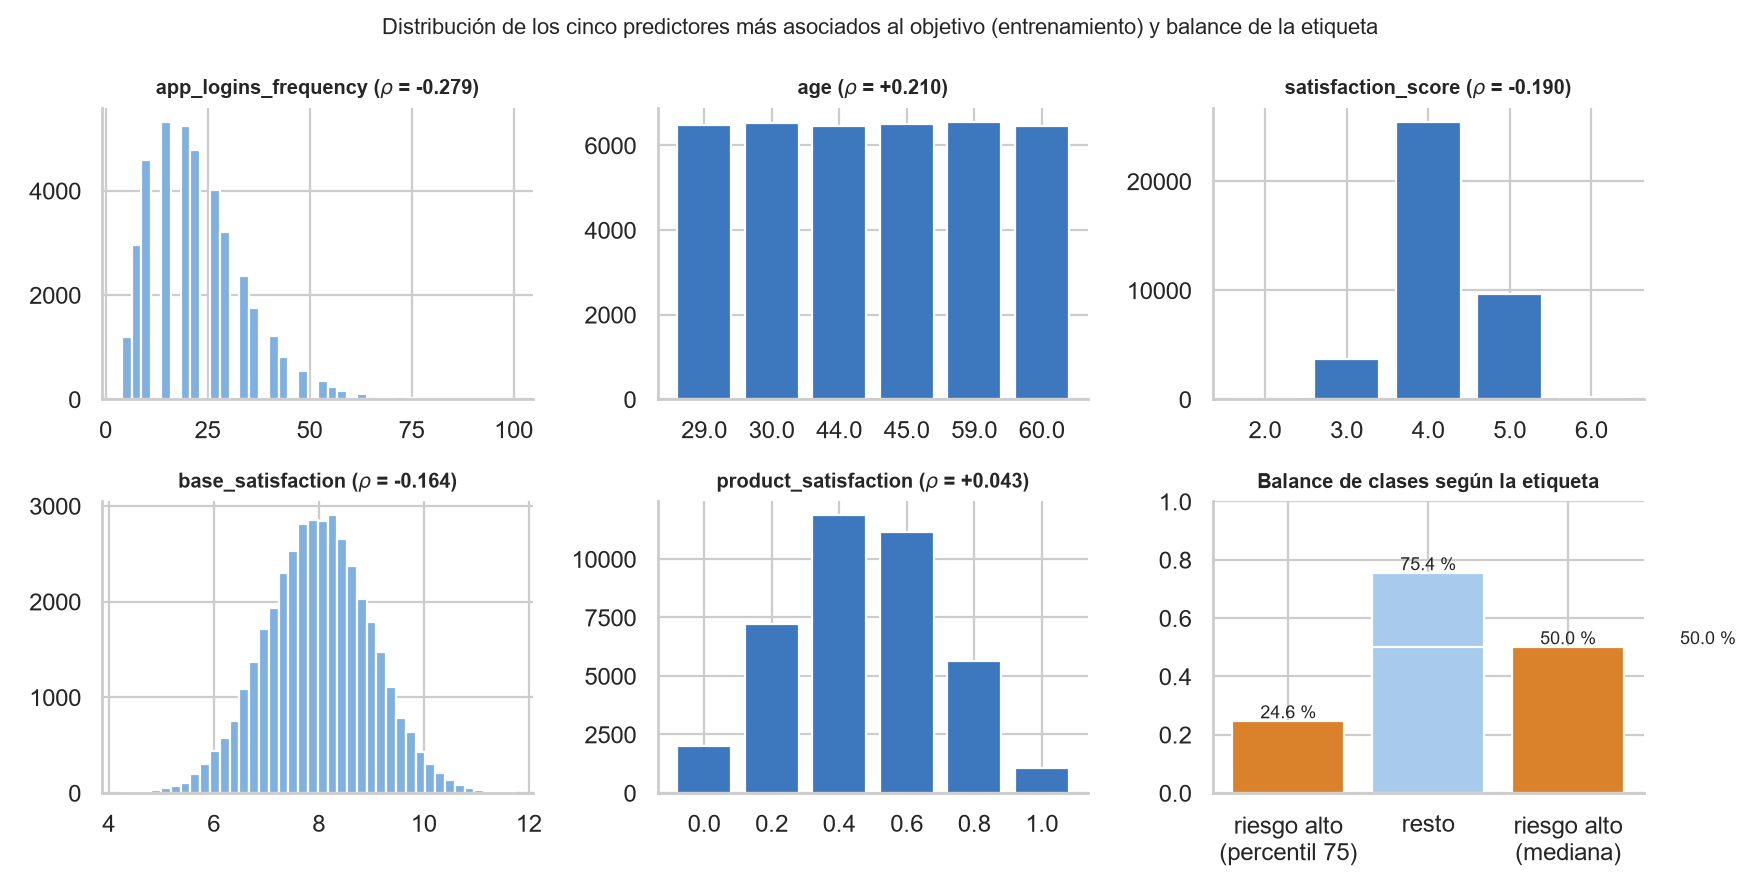
\includegraphics[width=\textwidth]{eda_univariado.png}
\caption{Distribución en el entrenamiento de los cinco predictores más asociados al objetivo (con la $\rho$ de Spearman con \cp) y balance de clases de la etiqueta de riesgo alto con el percentil 75 (la de este trabajo) y con la mediana (la de la entrega anterior).}\label{fig:univariado}
\end{figure}

\begin{figure}[htbp]
\centering
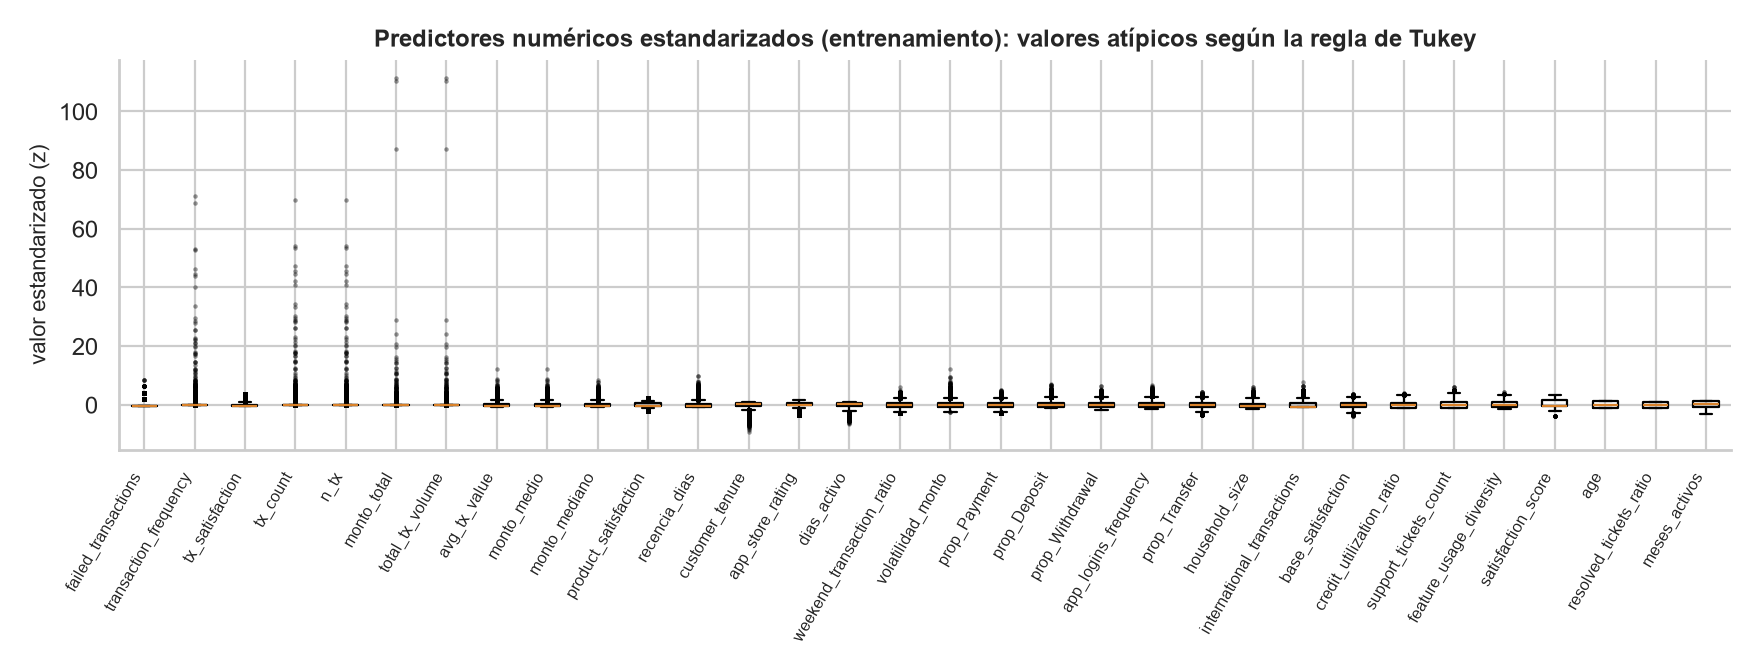
\includegraphics[width=\textwidth]{eda_boxplots.png}
\caption{Diagramas de caja de los predictores numéricos estandarizados en el entrenamiento, ordenados por proporción de valores atípicos según la regla de Tukey.}\label{fig:boxplots}
\end{figure}

El análisis bivariado explica el fracaso de los modelos lineales y es la raíz de la propuesta. La correlación más fuerte con el objetivo es la de \ap: $r=-0{,}876$, y esa sola variable explica el 76,8\,\% de la varianza. Su media desciende en una escalera de saltos casi idénticos ($-0{,}0498$, $-0{,}0496$, $-0{,}0508$ y $-0{,}0496$; desviación entre saltos 0,0006) con la misma dispersión en cada nivel (Figura~\ref{fig:objetivo}, derecha). Un paso constante es la firma de una regla de generación, no de una asociación empírica: el puntaje se construyó a partir del número de productos activos. Un modelo que conoce esa variable explica el 99,9\,\% del objetivo, pero no predice la fuga, sino que recupera la fórmula; por eso \ap\ se excluye como predictor, siguiendo la noción de fuga de información de \cite{kaufman2012leakage}. Sin ella, la señal se concentra en cuatro variables (Figura~\ref{fig:senal}): \texttt{app\_logins\_frequency} ($\rho=-0{,}279$), \texttt{age} ($+0{,}210$), \texttt{satisfaction\_score} ($-0{,}190$) y \texttt{base\_satisfaction} ($-0{,}164$); las doce variables transaccionales no aportan ($|\rho|\le0{,}018$). Y las relaciones no son lineales: la frecuencia de uso reduce el riesgo con fuerza al principio y luego se aplana, la satisfacción lo baja por escalones y la satisfacción de base lo hace en forma de S. La matriz de correlación (Figura~\ref{fig:correlacion}) muestra que las dos satisfacciones miden aspectos parecidos ($\rho=0{,}83$) y que \texttt{n\_tx}, derivada del detalle, duplica a \texttt{tx\_count} ($\rho=1{,}00$); se conservó para que todas las corridas usen las mismas columnas, sin efecto en los resultados.

\begin{figure}[htbp]
\centering
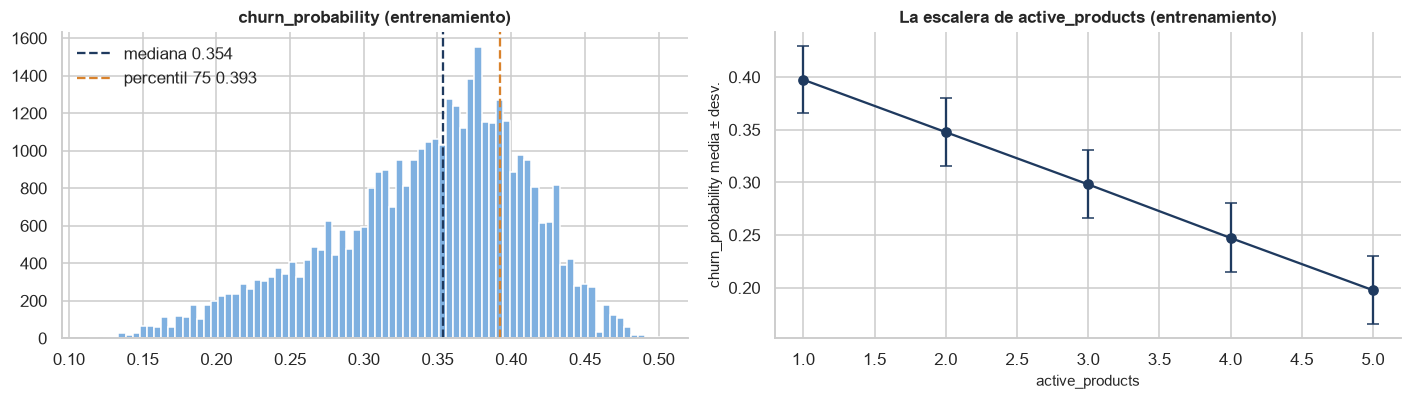
\includegraphics[width=\textwidth]{objetivo_escalera.png}
\caption{Izquierda: distribución de \cp\ en el entrenamiento con los umbrales de la mediana y del percentil 75. Derecha: media y desviación de \cp\ por número de productos activos, con la escalera de paso constante que delata la regla de generación del puntaje.}\label{fig:objetivo}
\end{figure}

\begin{figure}[htbp]
\centering
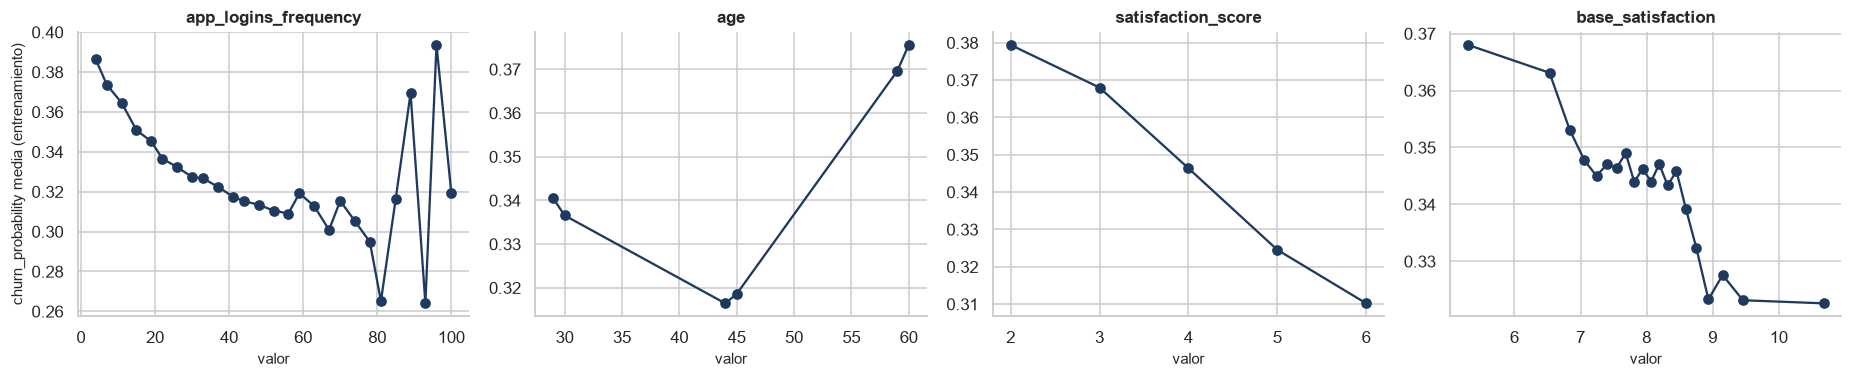
\includegraphics[width=\textwidth]{senal_bivariado.png}
\caption{Media de \cp\ en el entrenamiento según el valor de cada una de las cuatro variables con señal: los efectos se aplanan, cambian por tramos o siguen una curva en S, lo que una relación lineal no puede representar.}\label{fig:senal}
\end{figure}

\begin{figure}[htbp]
\centering
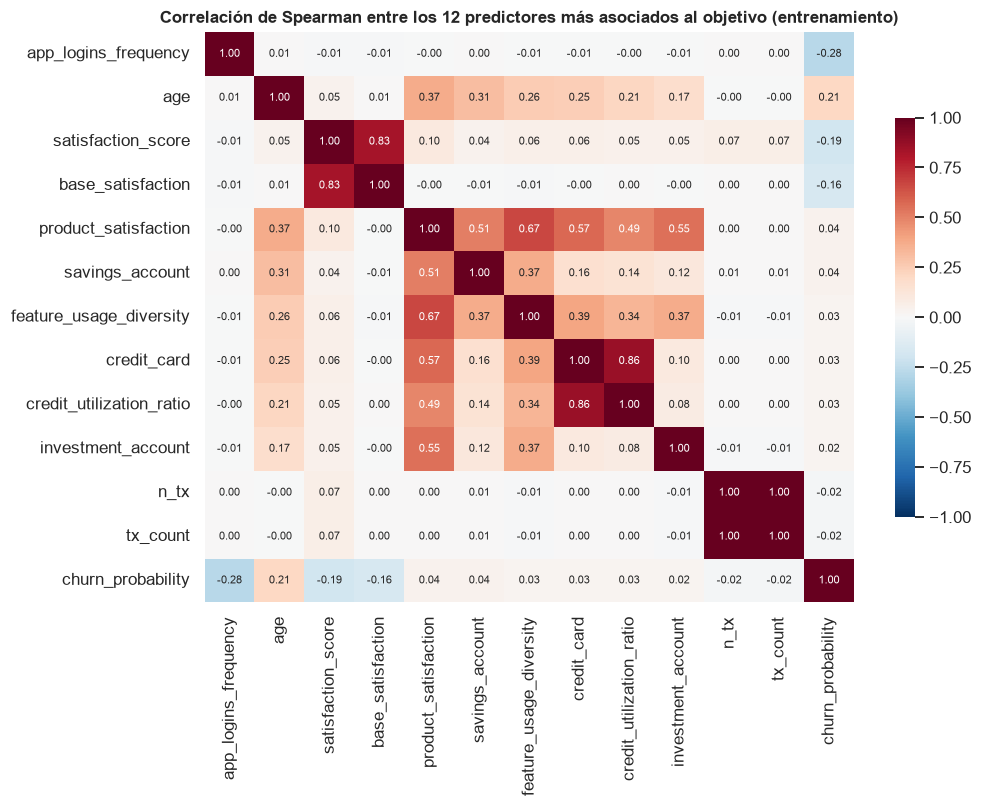
\includegraphics[width=0.8\textwidth]{correlacion.png}
\caption{Correlación de Spearman entre los doce predictores más asociados al objetivo y \cp\ (entrenamiento).}\label{fig:correlacion}
\end{figure}

\paragraph{Conclusiones del EDA y decisiones de preprocesamiento.}
Como consecuencia directa de lo observado: (1) se excluyó \ap\ y se midió el techo de información que deja su ausencia (Sección~\ref{sec:config}); (2) se eligió la etiqueta del percentil 75, porque con la mediana las clases quedan al 50\,\% por construcción y las técnicas de balanceo no tienen nada que hacer (ADASYN no genera ningún cliente sintético); (3) la partición es aleatoria y no por posición, porque el archivo está ordenado por cohortes; (4) las pruebas que dependen del orden de las filas (Ljung-Box, BDS, bootstrap estacionario) se calculan en el orden original del archivo, que induce dependencia entre vecinos; (5) la no linealidad de los cuatro predictores con señal motiva el modelo propuesto, que representa cada efecto con una función de forma libre; y (6) la colinealidad entre las dos satisfacciones se deja a la regularización de cada modelo, en lugar de eliminar una de ellas a mano.

\subsection{Modelos SOTA de referencia (\textit{baselines})}\label{sec:baselines}

El modelo propuesto se compara con todos los modelos del curso, en las dos tareas: k vecinos más cercanos, Naive Bayes gaussiano, regresión logística con penalización L1 y L2, Ridge y Lasso, árbol de decisión, Random Forest, XGBoost y máquinas de vectores de soporte (SVM y SVR), en su implementación de scikit-learn \cite{pedregosa2011sklearn} salvo XGBoost, más los dos modelos de la entrega anterior reentrenados con sus hiperparámetros. Cada modelo se describe una sola vez en el código con una rejilla explícita para Grid Search y un espacio tipado (escala logarítmica para $C$, $\alpha$ y las tasas de aprendizaje; enteros en escala logarítmica para vecinos y tamaños de hoja) para los otros tres métodos; las Tablas~\ref{tab:espacios_clasificacion} y~\ref{tab:espacios_regresion} recogen los espacios y los hiperparámetros finales. Dentro de cada modelo los cuatro métodos reciben el mismo presupuesto: tantas evaluaciones como puntos tiene su rejilla (entre 30 y 48). Sea $\{(x_i,y_i)\}_{i=1}^n$ el entrenamiento, con $x_i\in\mathbb{R}^p$ ($p=78$ tras el preprocesamiento).

\paragraph{k vecinos más cercanos \cite{cover1967knn}.}
Es la referencia no paramétrica: no supone ninguna forma funcional y, con suficientes datos, aproxima a la regla de Bayes. Con $N_k(x)$ el conjunto de los $k$ vecinos de $x$ según la distancia de Minkowski $d_q(x,x')=(\sum_j|x_j-x'_j|^q)^{1/q}$ y pesos $w_i=1$ (uniformes) o $w_i=1/d_q(x,x_i)$ (por distancia),
\begin{equation}
\hat{p}(y=1\mid x)=\frac{\sum_{i\in N_k(x)} w_i\,\mathbb{1}[y_i=1]}{\sum_{i\in N_k(x)} w_i},\qquad
\hat{f}(x)=\frac{\sum_{i\in N_k(x)} w_i\,y_i}{\sum_{i\in N_k(x)} w_i}.
\end{equation}
Se exploran $k\in[5,600]$ (escala logarítmica), el tipo de peso y $q\in\{1,2\}$; el entrenamiento solo guarda los datos y el coste se traslada a la consulta, $O(n\,p)$ por cliente en fuerza bruta, que en 78 dimensiones no mejora con árboles KD o Ball (Sección~\ref{sec:res_computo}). No admite ponderación de clases porque su predicción es un voto sin función de pérdida.

\paragraph{Naive Bayes gaussiano \cite{hand2001naivebayes}.}
Es el modelo generativo más simple y sirve de cota inferior: supone independencia condicional entre las 78 columnas,
\begin{equation}
\hat{y}=\arg\max_{c\in\{0,1\}}\ \pi_c\prod_{j=1}^{p}\mathcal{N}\!\left(x_j;\,\mu_{jc},\,\sigma^2_{jc}+\varepsilon\,\max_{j'}\sigma^2_{j'}\right),
\end{equation}
donde $\varepsilon$ (\texttt{var\_smoothing}, en escala logarítmica) estabiliza las varianzas y la ponderación de clases equivale a fijar $\pi_0=\pi_1=1/2$. Entrena en $O(n\,p)$.

\paragraph{Regresión logística regularizada \cite{tibshirani1996lasso,hoerl1970ridge}.}
Es la línea base lineal y el modelo de clasificación de la entrega anterior. Con $y_i\in\{-1,+1\}$ y mezcla $\lambda\in\{0,1\}$ entre Ridge ($\lambda=0$) y Lasso ($\lambda=1$),
\begin{equation}
\min_{\beta,b}\ \sum_{i=1}^{n}\log\!\left(1+e^{-y_i(\beta^\top x_i+b)}\right)+\frac{1}{C}\left[\lambda\|\beta\|_1+\frac{1-\lambda}{2}\|\beta\|_2^2\right],
\end{equation}
resuelto con liblinear; se exploran $C\in[10^{-3},10^{2}]$ (log) y $\lambda$. La penalización L1 selecciona variables y la L2 reparte el peso entre columnas correlacionadas. La ponderación de clases multiplica cada término de la suma por $w_{y_i}=n/(2n_{y_i})$.

\paragraph{Ridge y Lasso \cite{hoerl1970ridge,tibshirani1996lasso}.}
Son los modelos de regresión de la entrega anterior:
\begin{equation}
\hat\beta_{\mathrm{ridge}}=\arg\min_\beta\ \|y-X\beta\|_2^2+\alpha\|\beta\|_2^2,\qquad
\hat\beta_{\mathrm{lasso}}=\arg\min_\beta\ \frac{1}{2n}\|y-X\beta\|_2^2+\alpha\|\beta\|_1,
\end{equation}
con $\alpha\in[10^{-3},10^{5}]$ y $\alpha\in[10^{-5},10^{-1}]$ (log), rangos que cubren ambos lados de los óptimos de la entrega anterior (1000 y $10^{-4}$). Ridge se resuelve de forma directa (Cholesky) y Lasso por descenso por coordenadas; ambos son lineales en $n$.

\paragraph{Árbol de decisión \cite{breiman1984cart}.}
Representa la familia no lineal más simple y el componente de los ensambles. CART elige en cada nodo la partición $(j,s)$ que minimiza la impureza ponderada de los hijos, $\sum_{h\in\{L,R\}}\frac{n_h}{n}\,I(h)$, con la impureza de Gini $I=1-\sum_c \hat p_c^2$ (o la entropía) en clasificación y el error cuadrático medio en regresión, y se poda por coste-complejidad minimizando $R_\gamma(T)=R(T)+\gamma|T|$. Se exploran la profundidad máxima, el mínimo de observaciones por hoja (escala logarítmica hasta 300) y $\gamma$ (\texttt{ccp\_alpha}, log). Entrena en $O(n\,p\log n)$ y predice en $O(d)$.

\paragraph{Random Forest \cite{breiman2001rf}.}
Promedia $T$ árboles, cada uno ajustado sobre una muestra bootstrap y con un subconjunto aleatorio de \texttt{max\_features} variables en cada partición, lo que decorrelaciona los árboles y reduce la varianza:
\begin{equation}
\hat{f}_{\mathrm{RF}}(x)=\frac{1}{T}\sum_{t=1}^{T} f_t(x).
\end{equation}
$T$ no se optimiza, porque el error decrece de forma monótona con $T$ y se estabiliza; se aplica multi-fidelidad: la búsqueda evalúa cada configuración con 100 árboles y el modelo final usa 300. Se exploran \texttt{max\_features}, la profundidad y el mínimo por hoja.

\paragraph{XGBoost \cite{chen2016xgboost}.}
Es el \textit{gradient boosting} de referencia en datos tabulares y el mejor modelo visto en clase en este problema. En la iteración $t$ añade el árbol $f_t$ que minimiza la aproximación de segundo orden de la pérdida regularizada,
\begin{equation}
\mathcal{L}^{(t)}=\sum_{i=1}^{n}\left[g_i f_t(x_i)+\tfrac{1}{2}h_i f_t^2(x_i)\right]+\gamma\,|T_t|+\tfrac{\lambda}{2}\|w_t\|_2^2,
\end{equation}
con $g_i$ y $h_i$ el gradiente y la hessiana de la pérdida en la predicción acumulada, $|T_t|$ el número de hojas y $w_t$ sus valores. Se exploran la tasa de aprendizaje y el número de árboles (ambos en log, porque interactúan), la profundidad, \texttt{subsample}, \texttt{colsample\_bytree}, $\lambda$ y \texttt{min\_child\_weight}; el método de construcción es \texttt{hist}, siete veces más rápido que el exacto con el mismo AUC (Sección~\ref{sec:res_computo}). La ponderación de clases usa \texttt{scale\_pos\_weight} igual al cociente negativos/positivos del pliegue.

\paragraph{SVM y SVR \cite{cortes1995svm}.}
Con $n\approx39.000$ el SVM con núcleo es cuadrático o cúbico en $n$ (se extrapola en la Sección~\ref{sec:res_computo}), de modo que el modelo de referencia es el lineal en su formulación primal con pérdida de bisagra al cuadrado y penalización L2,
\begin{equation}
\min_{w,b}\ \tfrac{1}{2}\|w\|_2^2+C\sum_{i=1}^{n}\max\!\big(0,\,1-y_i(w^\top x_i+b)\big)^2,
\end{equation}
y, en regresión, con la pérdida $\varepsilon$-insensible al cuadrado, $\max(0,|y_i-w^\top x_i-b|-\varepsilon)^2$. Se exploran $C\in[10^{-4},10^{2}]$ y, en SVR, $\varepsilon\in[10^{-4},5\cdot10^{-2}]$ (la desviación típica del objetivo es 0,067). Medido sobre un pliegue interno, la penalización L1 y la pérdida $\varepsilon$-insensible lineal (solucionador dual) no convergían en 1.000 iteraciones, mientras que las variantes elegidas convergen en cuatro o cinco iteraciones y menos de un segundo.

\paragraph{Balanceo.}
Cada clasificador se entrena sin balanceo, con SMOTE \cite{chawla2002smote}, con ADASYN \cite{he2008adasyn} y con ponderación de clases (\texttt{class\_weight}); el sobremuestreo se ajusta solo con las filas de entrenamiento de cada pliegue y las combinaciones que no aplican (k-NN con ponderación) se registran como tales. En regresión no hay balanceo.

\begin{table}[htbp]
\caption{Espacios de búsqueda en clasificación: puntos de la rejilla de Grid Search (igual al presupuesto de los otros tres métodos), espacio tipado y hiperparámetros del modelo final de la mejor combinación.}\label{tab:espacios_clasificacion}
\tiny\setlength{\tabcolsep}{2pt}
\begin{tabular}{lr>{\raggedright\arraybackslash}p{4.7cm}>{\raggedright\arraybackslash}p{3.3cm}}
\toprule
\textbf{Modelo} & \textbf{Rejilla} & \textbf{Espacio de búsqueda} & \textbf{Hiperparámetros finales} \\
\midrule
k-NN & 32 & n\_neighbors $\in$ [5, 600] (entero log); weights $\in$ \{uniform, distance\}; p $\in$ \{1, 2\} & n\_neighbors=600, weights=distance, p=1 \\
Naive Bayes & 30 & var\_smoothing $\in$ [1e-11, 0.001] (log) & var\_smoothing=0.001 \\
Regresión logística & 30 & C $\in$ [0.001, 100] (log); l1\_ratio $\in$ \{1.0, 0.0\} & C=0.05631, l1\_ratio=1 \\
Árbol de decisión & 48 & max\_depth $\in$ [3, 30] (entero); min\_samples\_leaf $\in$ [1, 300] (entero log); ccp\_alpha $\in$ [1e-06, 0.01] (log); criterion $\in$ \{gini, entropy\} & ccp\_alpha=0.0003897, criterion=gini, max\_depth=22, min\_samples\_leaf=7 \\
Random Forest & 36 & max\_depth $\in$ [4, 40] (entero); max\_features $\in$ \{sqrt, log2, 0.3, 0.5\}; min\_samples\_leaf $\in$ [1, 100] (entero log) & max\_depth=32, max\_features=0.5, min\_samples\_leaf=11, n\_estimators=300 \\
XGBoost & 32 & n\_estimators $\in$ [100, 1000] (entero log); max\_depth $\in$ [2, 10] (entero); learning\_rate $\in$ [0.001, 0.3] (log); subsample $\in$ [0.5, 1] (lineal); colsample\_bytree $\in$ [0.5, 1] (lineal); reg\_lambda $\in$ [0.01, 10] (log); min\_child\_weight $\in$ [1, 50] (entero log) & n\_estimators=145, max\_depth=6, learning\_rate=0.003304, subsample=0.8081, colsample\_bytree=0.9683, reg\_lambda=0.8792, min\_child\_weight=11 \\
SVM lineal & 30 & C $\in$ [0.0001, 100] (log) & C=0.001083 \\
EBM & 36 & learning\_rate $\in$ [0.008, 0.1] (log); max\_leaves $\in$ [2, 4] (entero); min\_samples\_leaf $\in$ [2, 200] (entero log); interactions $\in$ [0, 20] (entero); max\_bins $\in$ [64, 1024] (entero log) & interactions=0, learning\_rate=0.008, max\_leaves=2, min\_samples\_leaf=100, outer\_bags=8 \\
\bottomrule
\end{tabular}
\end{table}

\begin{table}[htbp]
\caption{Espacios de búsqueda en regresión: puntos de la rejilla de Grid Search (igual al presupuesto de los otros tres métodos), espacio tipado y hiperparámetros del modelo final de la mejor combinación.}\label{tab:espacios_regresion}
\tiny\setlength{\tabcolsep}{2pt}
\begin{tabular}{lr>{\raggedright\arraybackslash}p{4.7cm}>{\raggedright\arraybackslash}p{3.3cm}}
\toprule
\textbf{Modelo} & \textbf{Rejilla} & \textbf{Espacio de búsqueda} & \textbf{Hiperparámetros finales} \\
\midrule
k-NN & 32 & n\_neighbors $\in$ [5, 600] (entero log); weights $\in$ \{uniform, distance\}; p $\in$ \{1, 2\} & n\_neighbors=80, p=1, weights=distance \\
Ridge & 30 & alpha $\in$ [0.001, 100000] (log) & alpha=613.9 \\
Lasso & 30 & alpha $\in$ [1e-06, 0.1] (log) & alpha=0.0001087 \\
Árbol de decisión & 48 & max\_depth $\in$ [3, 30] (entero); min\_samples\_leaf $\in$ [1, 300] (entero log); ccp\_alpha $\in$ [1e-08, 0.0001] (log) & max\_depth=13, min\_samples\_leaf=101, ccp\_alpha=1.811e-06 \\
Random Forest & 36 & max\_depth $\in$ [4, 40] (entero); max\_features $\in$ \{sqrt, log2, 0.3, 0.5\}; min\_samples\_leaf $\in$ [1, 100] (entero log) & max\_depth=8, max\_features=0.5, min\_samples\_leaf=50, n\_estimators=300 \\
XGBoost & 32 & n\_estimators $\in$ [100, 1000] (entero log); max\_depth $\in$ [2, 10] (entero); learning\_rate $\in$ [0.001, 0.3] (log); subsample $\in$ [0.5, 1] (lineal); colsample\_bytree $\in$ [0.5, 1] (lineal); reg\_lambda $\in$ [0.01, 10] (log); min\_child\_weight $\in$ [1, 50] (entero log) & n\_estimators=512, max\_depth=2, learning\_rate=0.02361, subsample=0.8025, colsample\_bytree=0.7268, reg\_lambda=0.2158, min\_child\_weight=31 \\
SVR lineal & 30 & C $\in$ [0.001, 100] (log); epsilon $\in$ [0.0001, 0.05] (log) & C=46.43, epsilon=0.0003846 \\
EBM & 36 & learning\_rate $\in$ [0.008, 0.1] (log); max\_leaves $\in$ [2, 4] (entero); min\_samples\_leaf $\in$ [2, 200] (entero log); interactions $\in$ [0, 20] (entero); max\_bins $\in$ [64, 1024] (entero log) & interactions=0, learning\_rate=0.008, max\_leaves=3, min\_samples\_leaf=20, outer\_bags=8 \\
\bottomrule
\end{tabular}
\end{table}


\subsection{Modelo propuesto}\label{sec:propuesto}

\paragraph{Formulación.}
La \textit{Explainable Boosting Machine} \cite{lou2012intelligible,lou2013ga2m}, en la implementación \texttt{interpret} \cite{nori2019interpretml}, es un modelo aditivo generalizado con interacciones por pares (GA$^2$M):
\begin{equation}\label{eq:ebm}
g\big(\mathbb{E}[y\mid x]\big)=\beta_0+\sum_{j=1}^{p} f_j(x_j)+\sum_{(j,k)\in\mathcal{I}} f_{jk}(x_j,x_k),
\end{equation}
donde $g$ es el enlace logit en clasificación y la identidad en regresión, $f_j$ son funciones de forma unidimensionales y $\mathcal{I}$ es un conjunto de $K$ pares seleccionado con el algoritmo FAST \cite{lou2013ga2m}. A diferencia de un GAM con \textit{splines}, cada $f_j$ es una función escalonada sobre una discretización de $x_j$ en \texttt{max\_bins} intervalos, aprendida por \textit{boosting} cíclico: en cada ronda se recorren las $p$ variables en orden y, para cada una, se ajusta un árbol de regresión de $L$ hojas (\texttt{max\_leaves}) y al menos $m$ observaciones por hoja (\texttt{min\_samples\_leaf}) \emph{solo sobre esa variable} al gradiente negativo de la pérdida en la predicción acumulada, y se añade escalado por una tasa $\eta$ pequeña,
\begin{equation}\label{eq:boosting}
f_j^{(r+1)}(x_j)=f_j^{(r)}(x_j)+\eta\,h_j^{(r)}(x_j),\qquad h_j^{(r)}=\arg\min_{h}\sum_{i=1}^{n} w_i\,\big(r_i^{(r)}-h(x_{ij})\big)^2,
\end{equation}
con $r_i^{(r)}=-\partial\ell(y_i,\hat s_i^{(r)})/\partial\hat s_i^{(r)}$ y $\hat s_i$ la predicción en la escala de $g$. La tasa baja hace que el orden de las variables no importe y reparte la señal compartida entre variables correlacionadas. El procedimiento se repite sobre $B$ submuestras (bolsas externas) y las funciones se promedian, $f_j=\frac{1}{B}\sum_b f_j^{(b)}$, lo que reduce su varianza y da un intervalo para cada tramo. La predicción de un cliente es una suma de $p+K$ búsquedas en tablas: cada término es legible y la inferencia cuesta $O(p+K)$ por cliente.

\paragraph{Adaptaciones.}
La librería no ofrece ponderación de clases; se implementó un envoltorio (\texttt{EBMConPesos}) que, cuando la corrida usa \texttt{class\_weight}, pasa a la EBM pesos $w_i=n/(2n_{y_i})$ por observación, de modo que la pérdida ponderada $\sum_i w_i\,\ell(y_i,\hat s_i)$ de la ecuación~\eqref{eq:boosting} equivale a la ponderación balanceada de scikit-learn. La búsqueda de hiperparámetros es multi-fidelidad: durante la búsqueda cada configuración se evalúa con $B=2$ bolsas y el modelo que se mide en el bucle externo y se guarda se reajusta con $B=8$; como las bolsas promedian pero no cambian la forma de cada función, el orden de las configuraciones se conserva, supuesto que se comprueba empíricamente (Sección~\ref{sec:res_computo}). El espacio de búsqueda es $\eta\in[0{,}008;\,0{,}1]$ (log; por debajo de 0,008 cada ajuste tarda el doble), $L\in\{2,3,4\}$, $m\in[2,200]$ (log), $K\in\{0,\dots,20\}$ (0 es un GAM puro) y \texttt{max\_bins}$\in[64,1024]$ (log). El Algoritmo~\ref{alg:ebm} resume el entrenamiento.

\begin{algorithm}[htbp]
\caption{Entrenamiento de la EBM con bolsas externas, pesos de clase y multi-fidelidad}\label{alg:ebm}
\begin{algorithmic}[1]
\Require entrenamiento $\{(x_i,y_i)\}_{i=1}^n$, pesos $w_i$ (1 sin balanceo; $n/(2n_{y_i})$ con \texttt{class\_weight}), bolsas $B$, tasa $\eta$, hojas $L$, mínimo por hoja $m$, pares $K$, intervalos \texttt{max\_bins}
\Ensure $\beta_0$, funciones de forma $f_j$ y $f_{jk}$
\State discretizar cada $x_j$ en \texttt{max\_bins} intervalos por cuantiles (una sola vez)
\For{$b=1,\dots,B$}
    \State tomar una submuestra de entrenamiento y reservar el resto como validación de la bolsa
    \State $f_j^{(b)}\gets0$ para todo $j$; $\hat s_i\gets\beta_0$ (logit de la media ponderada o media)
    \While{la pérdida ponderada en la validación de la bolsa mejore (parada temprana)}
        \For{$j=1,\dots,p$} \Comment{ciclo sobre las variables}
            \State $r_i\gets-\partial\ell(y_i,\hat s_i)/\partial\hat s_i$ para todo $i$
            \State ajustar un árbol $h$ de $L$ hojas y mínimo $m$ sobre $x_j$ al residuo $r$ con pesos $w_i$
            \State $f_j^{(b)}\gets f_j^{(b)}+\eta\,h$;\quad $\hat s_i\gets\hat s_i+\eta\,h(x_{ij})$
        \EndFor
    \EndWhile
    \State seleccionar con FAST los $K$ pares $(j,k)$ que más reducen el residuo y repetir el ciclo sobre ellos con los $f_j^{(b)}$ fijos
\EndFor
\State $f_j\gets\frac{1}{B}\sum_b f_j^{(b)}$ y $f_{jk}\gets\frac{1}{B}\sum_b f_{jk}^{(b)}$, centradas; $\beta_0\gets$ media de las predicciones
\State \textbf{búsqueda:} evaluar cada configuración con $B=2$ en la validación interna; \textbf{modelo final:} reajustar la ganadora con $B=8$
\end{algorithmic}
\end{algorithm}

\paragraph{Por qué debe funcionar aquí.}
La justificación es estructural. El EDA muestra que la señal está en pocas variables con efectos no lineales y que los pares de predictores son casi independientes (Figura~\ref{fig:correlacion}): esa es exactamente la hipótesis aditiva de la ecuación~\eqref{eq:ebm}, que puede representar escalones, mesetas y curvas en S sin necesidad de interacciones profundas. Frente a los modelos lineales, gana flexibilidad por variable; frente a XGBoost y Random Forest, restringe el espacio de hipótesis a sumas de funciones de una variable (y de pocos pares), lo que reduce la varianza en un problema con 39.000 filas y una señal débil, sin perder lo que esos ensambles captan, porque la relación verdadera es aditiva en primera aproximación. El promedio sobre bolsas estabiliza las curvas igual que el \textit{bagging} del Random Forest. En coste, la predicción es una suma de búsquedas en tablas, más barata que recorrer cientos de árboles o que calcular distancias a 39.000 clientes; el precio se paga en el entrenamiento, que recorre las $p$ variables en cada ronda, $O(B\,R\,p\,(n+\texttt{bins}))$ para $R$ rondas, y que, como se muestra en los resultados, es mayor que el de XGBoost. Finalmente, el modelo no necesita un explicador: cada $f_j$ es la explicación, lo que responde a la segunda limitación señalada en la introducción.

\subsection{Configuración experimental}\label{sec:config}

\paragraph{Validación anidada y optimizadores.}
Cada corrida es una validación cruzada anidada \cite{cawley2010overfitting}: un bucle externo de 5 pliegues (estratificados en clasificación, los mismos para todos los modelos) produce la única métrica que se reporta, y dentro de cada pliegue externo un bucle interno de 3 pliegues elige los hiperparámetros con uno de los cuatro métodos: Grid Search; Random Search sobre el espacio tipado; optimización bayesiana con el estimador Parzen estructurado en árbol (TPE) de Optuna \cite{akiba2019optuna}, que modela las densidades $\ell(x)$ del 10\,\% de configuraciones mejores y $g(x)$ del resto y propone el máximo de $\ell(x)/g(x)$, equivalente a la mejora esperada, tras 10 ensayos aleatorios; y un algoritmo genético con DEAP \cite{fortin2012deap} con genes en $[0,1]$, selección por torneo de 3, cruce uniforme (probabilidad 0,5 por gen, aplicado con 0,6), mutación gaussiana con $\sigma=0{,}15$ (1/$n$ por gen, aplicada con 0,3), elitismo, población $\max(4,\min(\text{presupuesto}/4,12))$, caché de genomas y diversidad registrada por generación. Al terminar, la misma búsqueda se repite sobre todo el entrenamiento y el ganador se reajusta con él: es el modelo final, que toca la prueba una sola vez. El mejor puntaje interno se guarda para medir el optimismo de selección, pero nunca se reporta.

\paragraph{Métricas.}
La métrica principal de clasificación es el AUC, porque no depende del umbral ni de la prevalencia y mide lo que necesita una campaña de retención con capacidad limitada: ordenar a los clientes por riesgo. Se reportan además el recall con umbral 0,5 (la métrica secundaria de la entrega anterior), el punto de operación que contacta al 25\,\% de mayor riesgo y la calibración (Brier y error de calibración esperado, con recalibración isotónica ajustada solo con predicciones fuera de pliegue). En regresión la métrica principal es el RMSE, en las unidades del objetivo, con $R^2$, e intervalos bootstrap BCa con 2.000 réplicas. Los residuos se someten a las pruebas de White, BDS, Ljung-Box y de normalidad.

\paragraph{Protocolo estadístico.}
En clasificación, Friedman con la corrección de Iman-Davenport sobre los pliegues externos y Nemenyi con diagrama de diferencia crítica \cite{demsar2006}; sobre la prueba, DeLong \cite{delong1988} por pares entre finalistas con corrección de Holm, y delta de Cliff. En regresión, el \textit{Model Confidence Set} al 90\,\% \cite{hansen2011mcs}, Diebold-Mariano \cite{diebold1995} con la corrección de Harvey-Leybourne-Newbold y bootstrap estacionario con longitud de bloque automática, y $d$ de Cohen. Las filas se toman en el orden original del archivo, que está organizado por bloques.

\paragraph{Techo de información.}
Para saber cuánto margen deja la exclusión de \ap, se entrena un oráculo (un \textit{gradient boosting} de histogramas) que sí la conoce y se promedia su pronóstico sobre la distribución de \ap\ del entrenamiento: es el mejor pronóstico posible sin conocerla, y se calcula sobre la misma prueba.

\paragraph{Hardware, software y tiempos.}
Todos los experimentos se ejecutaron en un equipo con procesador AMD de 6 núcleos, 15,9 GB de memoria, GPU NVIDIA GeForce RTX 3050 (6 GB) y Windows 11, con Python 3.13.3, scikit-learn 1.9.1, imbalanced-learn 0.14.2, XGBoost 3.4.1, interpret-core 0.7.8, Optuna 5.0.0 y DEAP 1.4.4. Las 140 corridas se ejecutaron en serie, con el equipo dedicado y el código congelado con su huella SHA-256, para que los tiempos por evaluación de los optimizadores no se contaminaran entre sí. El tiempo de cómputo se reporta de tres formas: la duración de cada corrida anidada completa (búsqueda $5\times3$ más modelo final), el tiempo de ajuste del modelo final sobre los 38.978 clientes de entrenamiento y el de inferencia sobre los 9.745 de prueba, estos dos como mediana de tres ajustes y cinco inferencias con el pipeline completo y el equipo sin otra carga. La sensibilidad a la semilla se midió reentrenando los modelos finales de Random Forest, XGBoost, SVM y la EBM con cinco a diez semillas, y repitiendo la búsqueda del árbol con cinco semillas de cada optimizador estocástico.

\section{Resultados}\label{sec:resultados}

\subsection{El modelo propuesto frente a todos los modelos de referencia}\label{sec:res_todos}

Las Tablas~\ref{tab:clasificacion} y~\ref{tab:regresion} comparan la mejor combinación de cada modelo, elegida por el bucle externo sin mirar la prueba, en métrica, y la Tabla~\ref{tab:tiempos}, en tiempo de cómputo. De las 140 combinaciones de la guía, 136 se entrenaron y 4 se registraron como \emph{no aplica} (k-NN con ponderación de clases); las 20 corridas de la EBM se añadieron con las mismas reglas. En clasificación con la etiqueta del percentil 75, la EBM obtiene el mayor AUC de prueba de los ocho modelos, por delante de XGBoost, Random Forest y el árbol de decisión, y en la validación anidada queda cuarta, a cuatro milésimas de XGBoost; las curvas ROC de la Figura~\ref{fig:roc} son casi indistinguibles entre los cuatro. Tres grupos aparecen con claridad: los modelos de árboles entre 0,825 y 0,833 de AUC externa, k-NN unas cinco centésimas por debajo, los dos lineales siete centésimas por debajo y Naive Bayes al final. El protocolo estadístico confirma que las diferencias dentro del primer grupo no son reales: Friedman sobre los pliegues externos rechaza la igualdad de los ocho modelos ($p<10^{-4}$), pero Nemenyi deja como finalistas a XGBoost, Random Forest, árbol y EBM (Figura~\ref{fig:cd}), y de sus seis parejas ninguna diferencia de AUC en la prueba (de 0,0006 a 0,0046) sobrevive a la corrección de Holm; los cuatro se separan con claridad de k-NN, de los lineales y de Naive Bayes. La validación anidada predijo la prueba casi sin sesgo: la correlación entre el AUC externo y el de prueba es 0,997 sobre las 124 corridas de clasificación, con una diferencia media de $+0{,}0016$. La variabilidad por semilla del AUC de prueba es de 0,0000 a 0,0010, del mismo orden que la diferencia entre la EBM y XGBoost (0,0006).

\begin{table}[htbp]
\caption{Clasificación (etiqueta del percentil 75): mejor combinación de balanceo y optimizador de cada modelo según el bucle externo, AUC externa (media $\pm$ desviación de los 5 pliegues) y AUC en la prueba (9.745 clientes). \emph{Pesos} es la ponderación de clases; los tiempos están en la Tabla~\ref{tab:tiempos}.}\label{tab:clasificacion}
\scriptsize\setlength{\tabcolsep}{2pt}
\begin{tabular}{lllrr}
\toprule
\textbf{Modelo} & \textbf{Balanceo} & \textbf{Optimizador} & \textbf{AUC externa} & \textbf{AUC prueba} \\
\midrule
XGBoost & pesos & Genética & 0,8332 $\pm$ 0,0049 & 0,8283 \\
Árbol de decisión & pesos & Random & 0,8332 $\pm$ 0,0021 & 0,8243 \\
Random Forest & -- & Genética & 0,8326 $\pm$ 0,0029 & 0,8260 \\
\textbf{EBM (propuesto)} & pesos & Grid & 0,8292 $\pm$ 0,0037 & 0,8289 \\
k-NN & -- & Genética & 0,7836 $\pm$ 0,0072 & 0,7874 \\
Regresión logística & pesos & Genética & 0,7644 $\pm$ 0,0047 & 0,7709 \\
SVM lineal & pesos & Grid & 0,7641 $\pm$ 0,0044 & 0,7706 \\
Naive Bayes & -- & Grid & 0,6722 $\pm$ 0,0119 & 0,6662 \\
\bottomrule
\end{tabular}
\end{table}

\begin{table}[htbp]
\caption{Regresión de \texttt{churn\_probability}: mejor optimizador de cada modelo según el bucle externo, RMSE externo (media $\pm$ desviación de los 5 pliegues) y RMSE y $R^2$ en la prueba.}\label{tab:regresion}
\scriptsize\setlength{\tabcolsep}{2pt}
\begin{tabular}{llrrr}
\toprule
\textbf{Modelo} & \textbf{Optimizador} & \textbf{RMSE externo} & \textbf{RMSE prueba} & \textbf{$R^2$ prueba} \\
\midrule
XGBoost & Bayesiana & 0,0590 $\pm$ 0,0004 & 0,0592 & 0,218 \\
\textbf{EBM (propuesto)} & Grid & 0,0590 $\pm$ 0,0004 & 0,0593 & 0,216 \\
Random Forest & Grid & 0,0592 $\pm$ 0,0004 & 0,0593 & 0,215 \\
Árbol de decisión & Genética & 0,0593 $\pm$ 0,0004 & 0,0594 & 0,211 \\
Lasso & Genética & 0,0618 $\pm$ 0,0005 & 0,0617 & 0,151 \\
Ridge & Genética & 0,0618 $\pm$ 0,0005 & 0,0617 & 0,151 \\
SVR lineal & Bayesiana & 0,0618 $\pm$ 0,0005 & 0,0617 & 0,150 \\
k-NN & Grid & 0,0634 $\pm$ 0,0004 & 0,0632 & 0,108 \\
\bottomrule
\end{tabular}
\end{table}

\begin{table}[htbp]
\caption{Tiempo de cómputo de la mejor combinación de cada modelo: ajuste del modelo final sobre los 38.978 clientes de entrenamiento y puntuación de los 9.745 de prueba (mediana de 3 y 5 repeticiones con el pipeline completo), y duración de la corrida anidada completa (búsqueda $5\times3$ más modelo final).}\label{tab:tiempos}
\scriptsize\setlength{\tabcolsep}{2pt}
\begin{tabular}{llrrr}
\toprule
\textbf{Tarea} & \textbf{Modelo} & \textbf{Ajuste (s)} & \textbf{Inferencia (s)} & \textbf{Corrida (min)} \\
\midrule
Clasificación & XGBoost & 1,61 & 0,060 & 8,9 \\
 & Árbol de decisión & 1,38 & 0,054 & 1,8 \\
 & Random Forest & 23,65 & 0,187 & 20,9 \\
 & \textbf{EBM (propuesto)} & 26,72 & 0,067 & 18,7 \\
 & k-NN & 0,28 & 7,164 & 34,7 \\
 & Regresión logística & 1,83 & 0,056 & 3,1 \\
 & SVM lineal & 0,92 & 0,052 & 2,1 \\
 & Naive Bayes & 0,30 & 0,068 & 0,7 \\
Regresión & XGBoost & 2,09 & 0,065 & 10,4 \\
 & \textbf{EBM (propuesto)} & 31,85 & 0,054 & 26,6 \\
 & Random Forest & 12,31 & 0,145 & 16,1 \\
 & Árbol de decisión & 0,84 & 0,047 & 3,7 \\
 & Lasso & 0,46 & 0,046 & 6,7 \\
 & Ridge & 0,28 & 0,046 & 1,5 \\
 & SVR lineal & 0,66 & 0,046 & 2,7 \\
 & k-NN & 0,25 & 4,725 & 24,9 \\
\bottomrule
\end{tabular}
\end{table}


\begin{figure}[htbp]
\centering
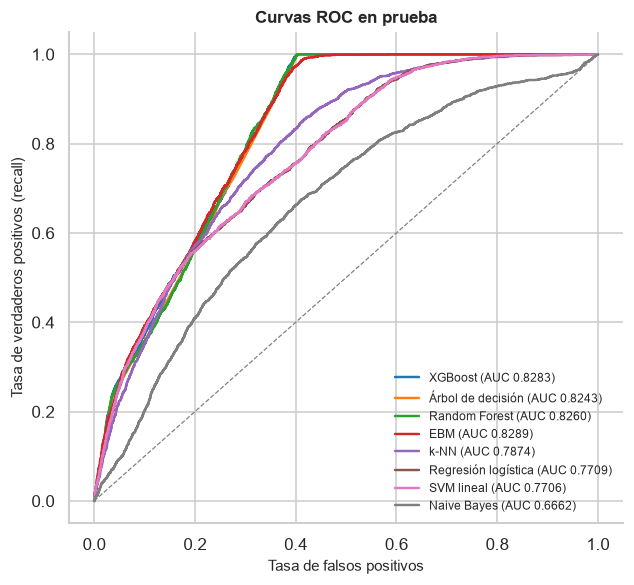
\includegraphics[width=0.55\textwidth]{roc.png}
\caption{Curvas ROC en la prueba (etiqueta del percentil 75) de la mejor combinación de cada modelo.}\label{fig:roc}
\end{figure}

\begin{figure}[htbp]
\centering
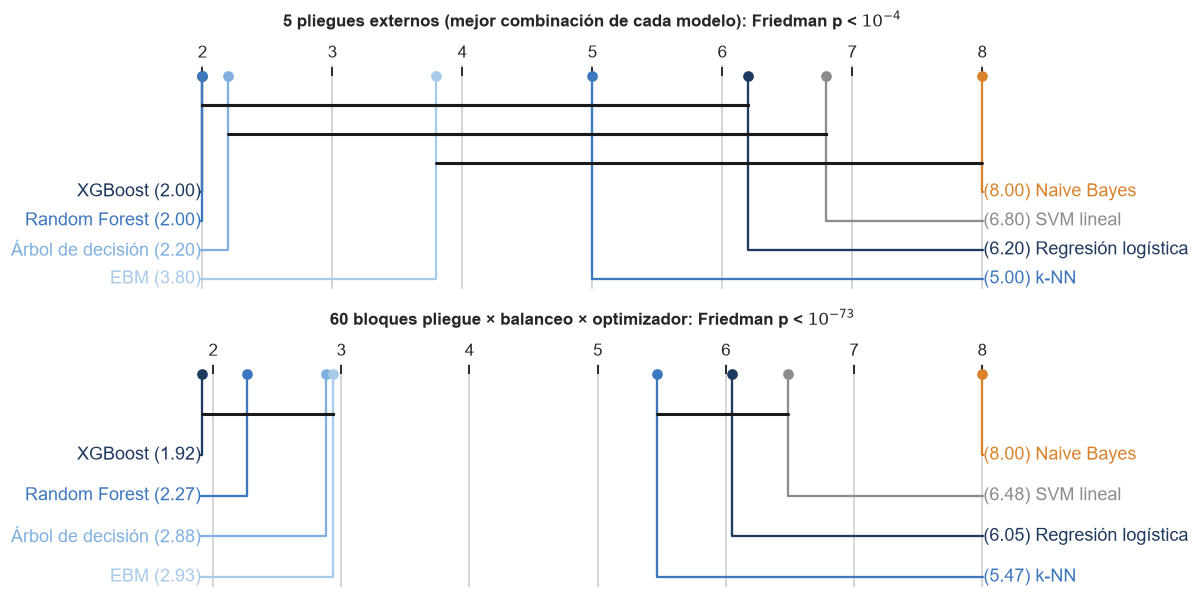
\includegraphics[width=0.9\textwidth]{cd_modelos.png}
\caption{Diagramas de diferencia crítica de Nemenyi sobre los 5 pliegues externos (arriba) y, como comprobación de robustez, sobre los 60 bloques pliegue $\times$ balanceo $\times$ optimizador (abajo); las barras unen modelos que no difieren al 5\,\%.}\label{fig:cd}
\end{figure}

En regresión, XGBoost y la EBM empatan en el RMSE externo (0,0590) y en la prueba la EBM queda segunda por una décima de milésima; el intervalo BCa de su RMSE se solapa con el de todos los modelos de árboles. Sin embargo, con 9.745 clientes las pérdidas de dos modelos están tan correlacionadas que diferencias sistemáticas de décimas de milésima son detectables: el \textit{Model Confidence Set} al 90\,\% se queda únicamente con XGBoost, y la EBM es el último modelo en salir ($p_{\mathrm{MCS}}=0{,}072$); Diebold-Mariano entre la EBM y XGBoost da $p=0{,}064$ (0,128 tras Holm) y el bootstrap estacionario, $p=0{,}069$. Los residuos de los modelos de árboles no muestran heterocedasticidad (White) ni dependencia en el orden del archivo (Ljung-Box y BDS); los de los lineales y k-NN sí conservan dependencia, porque no captan el efecto no lineal de la edad y su residuo hereda la estructura por cohortes; la normalidad se rechaza en todos, porque el residuo hereda la mezcla por niveles de \ap.

\paragraph{Tiempo de cómputo.}
Según la Tabla~\ref{tab:tiempos}, en inferencia la EBM está en el grupo más rápido: puntuar a los 9.745 clientes de prueba tarda unas 0,07 s en clasificación y 0,05 s en regresión, lo mismo que XGBoost y que los modelos lineales (el tiempo lo domina el preprocesado), casi tres veces menos que Random Forest con 300 árboles y cien veces menos que k-NN, cuya consulta calcula las distancias a los 38.978 clientes guardados; además, el modelo serializado ocupa 1,5 MB frente a los 44 MB del bosque de clasificación. En ajuste, en cambio, la EBM es el modelo más lento: 26,7 s en clasificación y 31,8 s en regresión sobre el entrenamiento completo, del orden de Random Forest (23,7 y 12,3 s) y entre 15 y 17 veces más que XGBoost (1,6 y 2,1 s), porque cada ronda de \textit{boosting} recorre las 78 columnas y el modelo final promedia 8 bolsas. La corrida anidada completa de la EBM tardó 18,7 min en clasificación, frente a 8,9 min de XGBoost, 20,9 de Random Forest y 34,7 de k-NN; con sobremuestreo, además, cada corrida de la EBM tardó 3,7 veces más que sin balanceo, sin ganancia alguna de AUC, de modo que sus 20 corridas sumaron 19,5 h frente a las 26,9 h de las 140 de la guía. El modelo propuesto no cumple, por tanto, el objetivo de ser también el más rápido de entrenar; sí cumple el de inferencia y el de tamaño, que son los que pesan en producción, donde el modelo se ajusta una vez y se consulta sobre toda la cartera.

\subsection{El modelo propuesto frente a la entrega anterior}\label{sec:res_e2}

Los modelos de la entrega anterior, reentrenados con este código, reproducen exactamente sus cifras publicadas (AUC 0,6832 y recall 0,6515; $R^2$ 0,1511 y RMSE 0,0617), de modo que el punto de partida es el mismo. La Tabla~\ref{tab:entrega2} resume la comparación en su partición, su etiqueta y su prueba, con la EBM y XGBoost afinados con el mismo protocolo (TPE, presupuesto de las 140 corridas, los mismos 5 pliegues), y la Tabla~\ref{tab:contrastes} recoge los contrastes. La EBM supera a la regresión logística en clasificación con una mejora de AUC de $+0{,}0355$, cuyo intervalo BCa no se acerca a cero y que DeLong confirma con $z=9{,}02$; gana además en los cinco pliegues de validación (delta de Cliff $+1$) y mejora el recall con umbral 0,5. En regresión supera al Lasso en $+0{,}0648$ de $R^2$, con Diebold-Mariano (HLN) de 13,3 y el bootstrap estacionario, que respeta la dependencia por bloques del archivo, en pleno acuerdo ($p<0{,}001$); la $d$ de Cohen por cliente es pequeña (0,135), porque la mejora de un cliente concreto es menor que el ruido de su pérdida, pero se repite en todos los pliegues ($d$ entre pliegues 6,1). Frente a XGBoost, el mejor modelo de clase, la EBM queda en $-0{,}0019$ de AUC y $-0{,}0017$ de $R^2$, sin diferencia significativa en ninguna de las dos tareas: empata con el mejor modelo de caja negra siendo un modelo legible.

\begin{table}[htbp]
\caption{Comparación con los modelos de la Entrega 2 en su misma partición, etiqueta (mediana estimada con el entrenamiento) y prueba. Cada modelo toca la prueba una sola vez; el techo es el mejor pronóstico posible sin \texttt{active\_products}.}\label{tab:entrega2}
\scriptsize\setlength{\tabcolsep}{2pt}
\begin{tabular}{lrrrr}
\toprule
\textbf{Modelo} & \textbf{AUC} & \textbf{Recall (0,5)} & \textbf{RMSE} & \textbf{$R^2$} \\
\midrule
Logística L1 (Entrega 2) & 0,6832 & 0,6515 & -- & -- \\
Lasso (Entrega 2) & -- & -- & 0,0617 & 0,1511 \\
XGBoost & 0,7206 & 0,6375 & 0,0592 & 0,2177 \\
\textbf{EBM (propuesto)} & 0,7187 & 0,6565 & 0,0593 & 0,2159 \\
Techo (oráculo) & 0,7223 & -- & -- & 0,2197 \\
\bottomrule
\end{tabular}
\end{table}

\begin{table}[htbp]
\caption{Contrastes sobre la prueba con la etiqueta de la mediana: diferencia de métrica del candidato con intervalo bootstrap BCa (2.000 réplicas), estadístico $z$ de DeLong para el AUC y DM de Diebold-Mariano con la corrección de Harvey-Leybourne-Newbold para la pérdida cuadrática, con $p$-valores ajustados por Holm.}\label{tab:contrastes}
\scriptsize\setlength{\tabcolsep}{2pt}
\begin{tabular}{llrlr}
\toprule
\textbf{Comparación} & \textbf{Métrica} & \textbf{$\Delta$ [IC BCa 95\,\%]} & \textbf{Estadístico} & \textbf{$p$ (Holm)} \\
\midrule
Logística (E2) $\rightarrow$ EBM & AUC & 0,0355 [0,0281; 0,0434] & $z$ = 9,02 & $<10^{-18}$ \\
Logística (E2) $\rightarrow$ XGBoost & AUC & 0,0374 [0,0303; 0,0449] & $z$ = 10,06 & $<10^{-22}$ \\
XGBoost $\rightarrow$ EBM & AUC & -0,0019 [-0,0051; 0,0009] & $z$ = -1,29 & 0,196 \\
Lasso (E2) $\rightarrow$ EBM & $R^2$ & 0,0648 [0,0551; 0,0738] & DM = 13,33 & $<10^{-39}$ \\
Lasso (E2) $\rightarrow$ XGBoost & $R^2$ & 0,0666 [0,0571; 0,0753] & DM = 14,05 & $<10^{-43}$ \\
XGBoost $\rightarrow$ EBM & $R^2$ & -0,0017 [-0,0036; 0,0003] & DM = -1,79 & 0,074 \\
\bottomrule
\end{tabular}
\end{table}


La Figura~\ref{fig:formas} muestra por qué falló la entrega anterior: el efecto de la edad en el logit va de $-0{,}73$ a $+0{,}85$ y no es monótono, el de la frecuencia de uso de la aplicación se aplana a partir de cierto nivel mientras la recta de la logística sigue bajando, y la penalización L1 había anulado \texttt{base\_satisfaction}, que en la EBM tiene un efecto claro en forma de S. Las cinco interacciones que eligió la EBM reúnen el 25,5\,\% de su importancia, pero una EBM idéntica sin interacciones obtiene 0,7185 de AUC frente a 0,7187 (DeLong $p=0{,}910$) y supera por sí sola a la entrega anterior: lo que faltaba era, sobre todo, flexibilidad en cada variable. El techo de información sin \ap\ es de 0,7223 de AUC y 0,2197 de $R^2$: la entrega anterior cubría el 82\,\% de la discriminación alcanzable (AUC $-0{,}5$) y el 69\,\% del $R^2$ alcanzable; la EBM llega al 98\,\% en ambos y XGBoost al 99\,\%. Queda, por tanto, muy poco margen, lo que explica el empate entre los dos.

\begin{figure}[htbp]
\centering
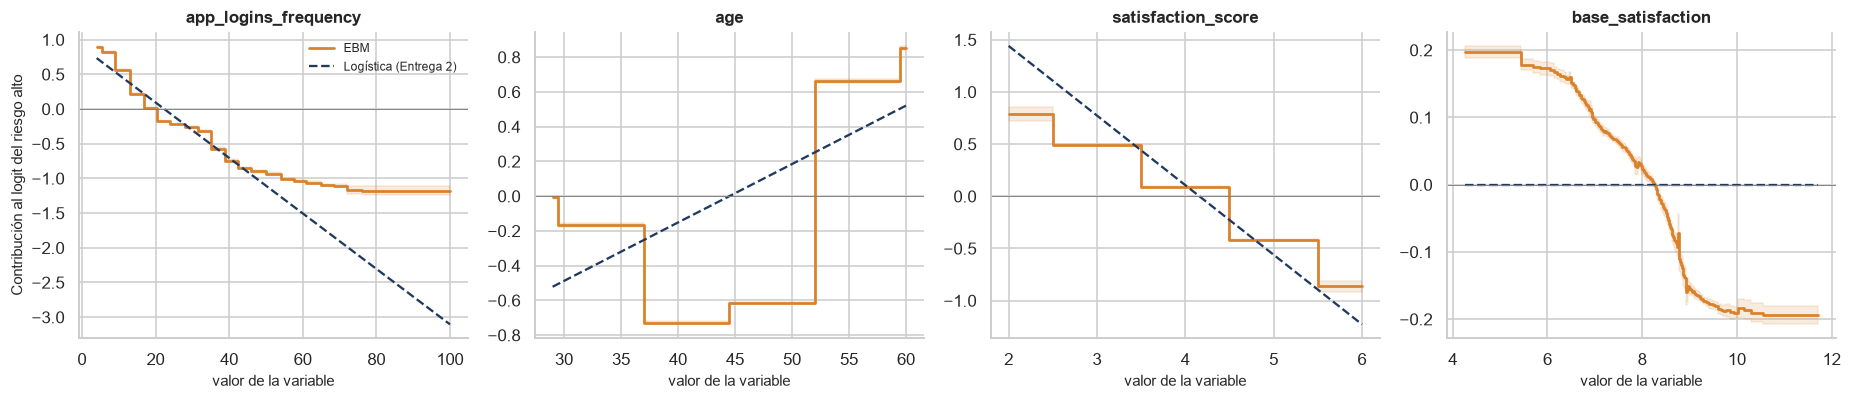
\includegraphics[width=\textwidth]{formas_ebm.png}
\caption{Funciones de forma de la EBM (contribución al logit del riesgo alto, con su intervalo entre bolsas) frente al efecto lineal que la logística L1 de la entrega anterior asigna a la misma variable, en la misma escala, para las cuatro variables con señal.}\label{fig:formas}
\end{figure}

\subsection{Optimización de hiperparámetros y cómputo}\label{sec:res_computo}

La Tabla~\ref{tab:optimizadores} compara los cuatro métodos con el mismo presupuesto. En la métrica final, genética, Grid y bayesiana terminan dentro de una fracción de milésima de AUC (Friedman $p=0{,}001$ en clasificación, sostenido únicamente por Random Search, que queda por debajo de Grid en el 74\,\% de los bloques, $-0{,}0019$ de AUC de media, Wilcoxon $p=0{,}004$); en regresión no hay diferencias ($p=0{,}815$). Lo que sí separa a los métodos es cuánto presupuesto necesitan: la optimización bayesiana tiene el menor rango medio del área bajo la curva de arrepentimiento normalizado en las dos tareas (Friedman $p<10^{-7}$ y $p<10^{-6}$), cierra el 95\,\% de la brecha en 10,3 evaluaciones frente a 14,2 de Grid, y Nemenyi la separa de Grid ($p<10^{-7}$), de Random ($p=0{,}028$) y de la genética ($p=0{,}001$); dentro de TPE, el 35\,\% de los ensayos guiados por el sustituto cae en el cuartil superior frente al 5\,\% de los ensayos aleatorios de arranque. La genética explora más (su diversidad cae de 0,274 a 0,078 en seis o siete generaciones sin colapsar) y termina con el mejor rango en la métrica externa de clasificación, pero es menos eficiente por evaluación. En tiempo de reloj la ventaja se invierte: por ser secuenciales, la bayesiana y la genética tardaron 1,7 veces más por evaluación en este equipo de 6 núcleos, porque solo paralelizan los 3 pliegues internos. El optimismo de selección salió negativo ($-0{,}0011$ de AUC en promedio): la validación interna subestima la externa porque entrena con menos filas, y los métodos adaptativos no muestran más sobreajuste que Grid. El balanceo, por su parte, no mejora la discriminación: la ponderación de clases deja el AUC igual (de $-0{,}0012$ a $+0{,}0009$) y SMOTE y ADASYN lo empeoran (hasta $-0{,}068$ en Naive Bayes; Friedman $p<10^{-10}$), porque el AUC mide el orden de los clientes y los clientes sintéticos añaden ruido en la frontera; lo que el balanceo mueve es el recall con el umbral de 0,5, es decir, el punto de operación.

\begin{table}[htbp]
\caption{Los cuatro métodos de optimización con el mismo presupuesto por modelo (27 bloques modelo $\times$ balanceo en clasificación y 7 en regresión): rango medio por la métrica externa (1 = mejor), bloques ganados, segundos por evaluación, área media bajo la curva de arrepentimiento normalizado (menor es mejor) y evaluaciones hasta cerrar el 95\,\% de la brecha.}\label{tab:optimizadores}
\scriptsize\setlength{\tabcolsep}{2pt}
\begin{tabular}{llrrrrr}
\toprule
\textbf{Tarea} & \textbf{Método} & \textbf{Rango medio} & \textbf{Victorias} & \textbf{s / eval.} & \textbf{Área arrep.} & \textbf{Evals. 95\,\%} \\
\midrule
Clasificación & Grid & 2,22 & 12 & 2,61 & 0,234 & 14,2 \\
 & Random & 3,22 & 4 & 2,46 & 0,171 & 7,2 \\
 & Bayesiana & 2,63 & 2 & 4,48 & 0,123 & 10,3 \\
 & Genética & 1,93 & 15 & 4,27 & 0,137 & 13,1 \\
Regresión & Grid & 2,71 & 2 & 2,43 & 0,181 & 9,9 \\
 & Random & 2,71 & 0 & 2,05 & 0,041 & 7,4 \\
 & Bayesiana & 2,14 & 2 & 2,94 & 0,038 & 5,5 \\
 & Genética & 2,43 & 3 & 3,37 & 0,057 & 7,4 \\
\bottomrule
\end{tabular}
\end{table}


La Tabla~\ref{tab:computo} resume los experimentos de optimización computacional que sostienen las decisiones del pipeline. El método \texttt{hist} de XGBoost entrena siete veces más rápido que el exacto con el mismo AUC y la GPU no acelera con 39.000 filas y árboles pequeños; con parada temprana el modelo se detiene en 153 árboles en lugar de 500, más rápido y con mejor AUC. En k-NN con 78 variables ni KD-Tree, ni Ball Tree ni FAISS mejoran la fuerza bruta, porque en alta dimensión un árbol apenas descarta regiones y las rutinas rápidas de FAISS son para la distancia euclídea, no para la Manhattan del modelo óptimo; lo que compensa es quedarse con las cuatro variables con señal, que bajan la consulta de 8,0 a 1,85 s y suben el AUC de 0,787 a 0,821. El SVM con núcleo RBF multiplicaría por 70 el coste de cada ajuste sin mejorar la métrica. La multi-fidelidad se valida con configuraciones aleatorias evaluadas con las dos fidelidades: la correlación de Spearman entre fidelidades es de 0,94 en Random Forest y 0,83 en la EBM, la configuración ganadora es la misma y la fidelidad baja ahorra el 65\,\% del tiempo de búsqueda. Paralelizar dentro de cada corrida (pliegues $\times$ configuraciones) aprovechó mejor los 6 núcleos (2,6 veces más rápido que en serie) que paralelizar entre modelos (1,5 veces); Random Forest con 6 hilos acelera 4,2 veces, y el perfil de una validación cruzada muestra que el 79\,\% del tiempo es el ajuste del modelo, no el preprocesado ni el remuestreo.

\begin{table}[htbp]
\caption{Versión estándar frente a versión optimizada, con los hiperparámetros finales en el equipo de referencia (6 núcleos, RTX 3050): tiempo de entrenamiento (en k-NN, de consulta sobre la prueba) y cambio en la métrica de prueba (AUC; RMSE en Ridge).}\label{tab:computo}
\scriptsize\setlength{\tabcolsep}{2pt}
\begin{tabular}{l>{\raggedright\arraybackslash}p{2.0cm}>{\raggedright\arraybackslash}p{2.2cm}rrrr}
\toprule
\textbf{Modelo} & \textbf{Estándar} & \textbf{Optimizada} & \textbf{$t$ est. (s)} & \textbf{$t$ opt. (s)} & \textbf{Acel.} & \textbf{$\Delta$ métrica} \\
\midrule
XGBoost & exact (CPU) & hist (CPU, 6 hilos) & 5,76 & 0,82 & 7,0 & -0,0014 \\
XGBoost & hist (CPU) & hist (GPU RTX 3050) & 0,82 & 0,86 & 0,96 & 0,0000 \\
XGBoost & 500 árboles fijos & parada temprana (153 árboles) & 2,72 & 1,41 & 1,9 & 0,0025 \\
k-NN (consulta) & fuerza bruta, 78 var. & KD-Tree, 78 var. & 8,04 & 24,07 & 0,33 & 0,0000 \\
k-NN (consulta) & fuerza bruta, 78 var. & FAISS IndexFlat, 78 var. & 8,04 & 11,95 & 0,67 & 0,0000 \\
k-NN (consulta) & fuerza bruta, 78 var. & KD-Tree, 4 var. con señal & 8,04 & 1,85 & 4,3 & 0,0339 \\
Ridge & SAGA & Cholesky & 15,082 & 0,079 & 191 & -0,0000 \\
Logística L1 & SAGA & liblinear & 19,40 & 1,27 & 15,3 & -0,0000 \\
SVM & SVC RBF (extrapolado) & LinearSVC primal L2 & 43,1 & 0,61 & 70 & -- \\
Random Forest & 1 hilo & 6 hilos & 78,5 & 18,6 & 4,2 & 0,0000 \\
EBM & búsqueda, fidelidad alta & búsqueda, fidelidad baja & 306,6 & 105,7 & 2,9 & 0,0000 \\
Random Forest & búsqueda, fidelidad alta & búsqueda, fidelidad baja & 280,1 & 97,6 & 2,9 & 0,0000 \\
\bottomrule
\end{tabular}
\end{table}


\subsection{Calibración, punto de operación e interpretabilidad}

Con el umbral de 0,5 las métricas varían de un extremo a otro aunque el AUC sea parecido (el recall va de 0,000 en k-NN a 1,000 en el árbol), porque los modelos entrenados con ponderación de clases desplazan sus probabilidades hacia arriba. Fijando la capacidad de la campaña en el 25\,\% de clientes de mayor riesgo, la EBM captura el 51\,\% de la fuga con una precisión del 50\,\%, 2,05 veces lo que se obtendría al azar, con XGBoost y los lineales a milésimas. Sin recalibrar, el error de calibración esperado va de 0,027 (Random Forest) a 0,682 (Naive Bayes); la recalibración isotónica, ajustada solo con predicciones fuera de pliegue, lo deja entre 0,003 y 0,010 en todos los modelos sin cambiar su AUC, porque es monótona. En interpretabilidad, SHAP \cite{lundberg2017shap} sobre XGBoost atribuye el 97\,\% de la contribución a las mismas cuatro variables que el EDA y la EBM señalan (edad 43\,\%, frecuencia de uso 36\,\%, satisfacción 16\,\% y satisfacción de base 1\,\%), y la dependencia de los valores SHAP con cada variable reproduce la forma de las curvas de la EBM: para este problema la EBM da la explicación global sin coste adicional y con la misma capacidad predictiva.

\section{Conclusiones}\label{sec:conclusiones}

El modelo propuesto cumplió el objetivo en la dimensión de la precisión y solo en parte en la del tiempo de cómputo. La EBM superó con holgura y con significación estadística a los dos modelos de la entrega anterior en las dos tareas, obtuvo el mayor AUC de prueba entre todos los modelos del curso y empató estadísticamente con XGBoost, Random Forest y el árbol de decisión, que ningún contraste logra separar entre sí; en regresión quedó segunda, a una distancia que el \textit{Model Confidence Set} detecta pero que es de décimas de milésima de RMSE. Ese empate no es una debilidad del modelo sino una propiedad de los datos: sin la variable con la que se construyó el objetivo existe un techo de información del que la EBM y XGBoost quedan a pocas milésimas, y ningún modelo, por complejo que sea, puede superarlo con las variables disponibles. En tiempo, la EBM es tan rápida como el mejor modelo en inferencia y mucho más ligera en disco, pero es la más lenta de ajustar, varias veces más que XGBoost; para una campaña de retención, que ajusta el modelo una vez y lo consulta sobre toda la cartera, el coste relevante es el de inferencia, pero el resultado se reporta tal cual. Lo que la EBM añade frente a los ensambles con los que empata es la legibilidad: cada variable aporta una curva que se puede auditar y que muestra directamente la no linealidad que los modelos lineales no podían captar, sin necesidad de un explicador auxiliar. Del pipeline se desprenden además dos lecciones: la optimización bayesiana es la que mejor aprovecha cada evaluación aunque la métrica final no distinga a los métodos, y el balanceo no mejora la discriminación sino que elige el punto de operación, que conviene fijar por la capacidad de la campaña y recalibrar con regresión isotónica.

Entre las limitaciones del estudio: COFINFAD es un conjunto sintético (lo delatan las tres cohortes de edad, la escalera de productos activos y la ausencia de señal en las transacciones), el objetivo es el puntaje de otro modelo y no la fuga observada, de modo que lo que se aprende es a reproducir ese puntaje; se usó un único conjunto de datos y los tiempos corresponden a un solo equipo. Como trabajo futuro se propone validar en el tiempo con datos reales (entrenar con un periodo y probar con el siguiente), incorporar el coste de cada acción de retención para fijar el umbral, acelerar el ajuste de la EBM con una parada temprana más exigente o restringiendo las variables a las que tienen señal, como se mostró con k-NN, y explotar las secuencias de transacciones con modelos que las traten como series.

\section*{Declaraciones}

\begin{itemize}
\item \textbf{Disponibilidad de datos:} COFINFAD es público y puede descargarse de Mendeley Data (\url{https://data.mendeley.com/datasets/mhb4zn3258/1}, DOI 10.17632/mhb4zn3258.1, licencia CC BY 4.0); una copia comprimida de las dos tablas está en la carpeta \texttt{datos} del repositorio y el código la descomprime al cargarla.
\item \textbf{Disponibilidad de código:} el código completo (paquete \texttt{src}, guiones de las corridas, de la comparación con la entrega anterior, de los experimentos de cómputo y de este artículo), la tabla maestra con las 160 corridas, las predicciones de prueba, los cuadernos ejecutados y el libro de Jupyter están en \url{https://github.com/RubenEsg/Prediccion-de-fuga-de-clientes-en-fintech}, con el libro publicado en \url{https://rubenesg.github.io/Prediccion-de-fuga-de-clientes-en-fintech/}. El entorno se fija con \texttt{requirements.txt} (versiones exactas) y la semilla del proyecto es 42.
\item \textbf{Contribución de los autores:} los tres autores diseñaron el estudio, ejecutaron los experimentos, analizaron los resultados y redactaron el manuscrito; todos revisaron y aprobaron la versión final.
\item \textbf{Conflicto de intereses:} los autores declaran no tener conflictos de interés.
\end{itemize}

\bibliography{sn-bibliography}

\end{document}
